% !TeX spellcheck = hu_HU
\let\oldthesubsection=\thesubsection
\renewcommand{\thesubsection}{\Roman{subsection}}

%A dolgozat olyan nyelvtechnológiai előfeldolgozó algoritmusokat mutat be, melyek hatékonyan képesek szövegek elemzésére agglutináló nyelvek esetén. 
%Vizsgálataimat magyar nyelvre végeztem, de a módszerek kidolgozása során törekedtem a nyelvfüggetlenségre. 
%Így, a bemutatott eljárások más, hasonló struktúrájú nyelvek esetén is sikerrel alkalmazhatóak.
%Munkám során kiemelt szerep jutott a morfológiai egyértelműsítés feladatának, mivel ennek kimenetére számtalan információkinyerő rendszer épít.

%Az első téziscsoportban a általános magyar nyelvű morfológiai egyértelműsítés területén elért eredményeimről számolok be. 
%Ezt követően bemutatom a létrehozott annotáló eszköz egy gyakorlati alkalmazását. 
%Végül, ismertetem azon új előfeldolgozó eljárásokat, melyek zajos (klinikai) szövegeket is hatékonyan képesek elemezni.

\subsection{Hatékony morfológiai egyértelműsítő algoritmusok}
\label{thes:morf}

A morfológiai egyértelműsítés egy olyan összetett feladat, amely a szófaji címkék meghatározásából és a szavak töveinek azonosításából áll. 
Míg az első részfeladatot a szakirodalom megoldottnak tekinti, addig az utóbbi területen sokkal kevesebb fejleményről számolhatunk be. 
A téziscsoport először egy szótövező módszert ismertet, majd leírja a teljes morfológiai egyértelműsítés során létrehozott algoritmusokat.

\begin{core}
\begin{thesis}\label{thes:morf-lemma}
Kidolgoztam egy olyan metódust, ami agglutináló nyelvek, így magyar esetén is nagy pontossággal képes szavak lemmáit azonosítani. 
Az eljárás a tanítóanyagban látott szavakon túl az ún. ismeretlen szóalakokat is képes hatékonyan kezelni, amihez a morfológiai elemző lehetséges elemzésein kívül a tanítóanyagból épített statisztikai modellekre is épít. 
Mérésekkel kimutattam, hogy a módszer magyar nyelv esetén kimagasló pontossággal bír. 
\end{thesis} 

\begin{pub}
\cite{Orosz2011,Orosz2012,Orosz2012a,Orosz2013a}
\end{pub}
\end{core}

A létrehozott algoritmus két fázisban végzi a szótövesítést. 
Első lépésben meghatározza a szavak lehetséges lemmáinak halmazát, amihez felhasználja a morfológiai elemző javaslatait illetve egy ismeretlenszó-elemző kimenetét is. 
Ezt követően a jelölteket ($l$)  rangsorolja a szóalak ($w$) és az előzetesen kalkulált morfoszintaktikai címke ($t$) függvényében számolt valószínűségi értékek alapján:
\begin{equation}\label{lemma-interpolated}
S(l|w,t) = P(l)^{\lambda_1} P(l,t|w)^{\lambda_2}
\end{equation}
Az így kapott algoritmus egy egyszerű szótő gyakorisági eloszlást és egy szóvég-alapú valószínűségi modellt kombinálva határozza meg a legmegfelelőbb lemmát.
Ehhez a bemutatott eljárás az egyes összetevők javaslatainak helyességét vizsgálva hangolja a  $\lambda_i$ paraméterek értékét.

Méréseimmel megmutattam, hogy az új szótövező algoritmus kiemelkedő pontossággal bír magyar nyelv esetén. 

\thesisline%%%%%%%%%%%%%%%%%%%%%%%%%%%%%%%%%%%%%%%%%%%%%%%%%%%%%%%%%%%%%%%%%%%%%


\begin{core}
\begin{thesis}\label{thes:morf-tagging}
Létrehoztam egy olyan hibrid morfológiai egyértelműsítő eszközt (PurePos\footnote{A bemutatott rendszer szabadon elérhető a \href{https://github.com/ppke-nlpg/purepos}{https://github.com/ppke-nlpg/purepos} címen.}), mely hatékonyan alkalmazható  morfológiailag komplex és nyelvi erőforrásokban szegény nyelvek esetén. 
Az algoritmus statisztikai eljárásokra támaszkodva, morfológiai elemző integrált alkalmazásával és szabály alapú komponensek használatával hatékony egyértelműsítést tesz lehetővé. 
Az eszköz a szavak lemmáinak meghatározását a \ref{thes:morf-lemma} tézisben ismertetett módszerrel végzi.
Ezen kívül a rendszer architektúrája lehetőséget nyújt még domén specifikus szabályok hatékony alkalmazására is.
Megmutattam, hogy az eljárás magyar nyelv esetén state-of-the-art pontossággal rendelkezik (akár nagyon kevés tanítóanyag esetén is).
\end{thesis}

\begin{pub}
\cite{Orosz2011,Orosz2012,Orosz2012a,Orosz2013a}
\end{pub}
\end{core}

\begin{figure}[H] 
  \centering
  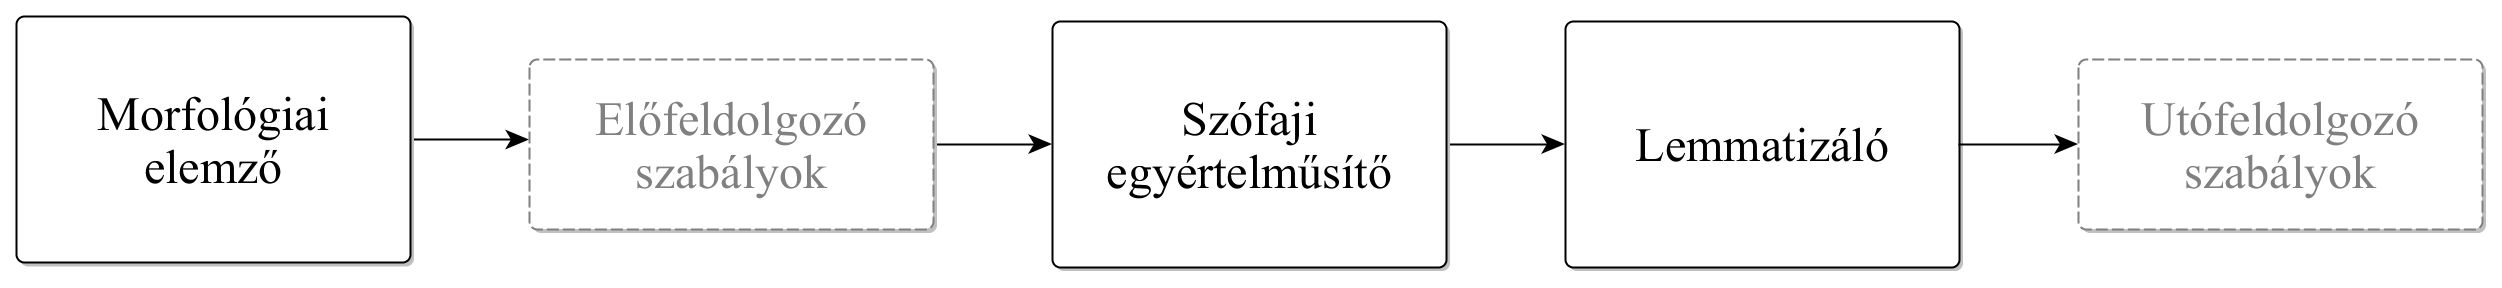
\includegraphics[width=1\textwidth]{MorphTagging/architecture_hu.png} 
  \caption{A hibrid morfológiai egyértelműsítő algoritmus architektúrája}
  \label{fig:purepos-arch_hu}
\end{figure}

A rendszer architektúráját  (ld. \ref{fig:purepos-arch_hu}. ábra) úgy alakítottam ki, hogy a statisztikai modulokon túl szimbolikus komponensekkel is hatékonyan tudjon együttműködni. 
Ily módon a címkék és szótövek azonosítása több lépésben történik:
az egyértelműsítés alapját egy morfológiai elemző képezi, melyet több lépésben sztochasztikus algoritmusok követnek. 
%Ezen eljárások elemző kimenetére épülve hozzák meg döntéseiket. 
%A szófaji egyértelműsítés folyamata olyan létező algoritmusokra épül, melyeket korábban már sikeresen használtak morfológiailag gazdag nyelvek elemzésére. 
A felhasznált trigram-alapú metódust úgy adaptáltam, hogy azok hatékonyan működjenek morfológiailag komplex nyelvek esetén is.
A szófaji címkézést követően, az elemzés utolsó fázisában történik a lemmák meghatározása a \ref{thes:morf-lemma} tézisben bemutatott módon.

\begin{figure} %[H]
  \centering
  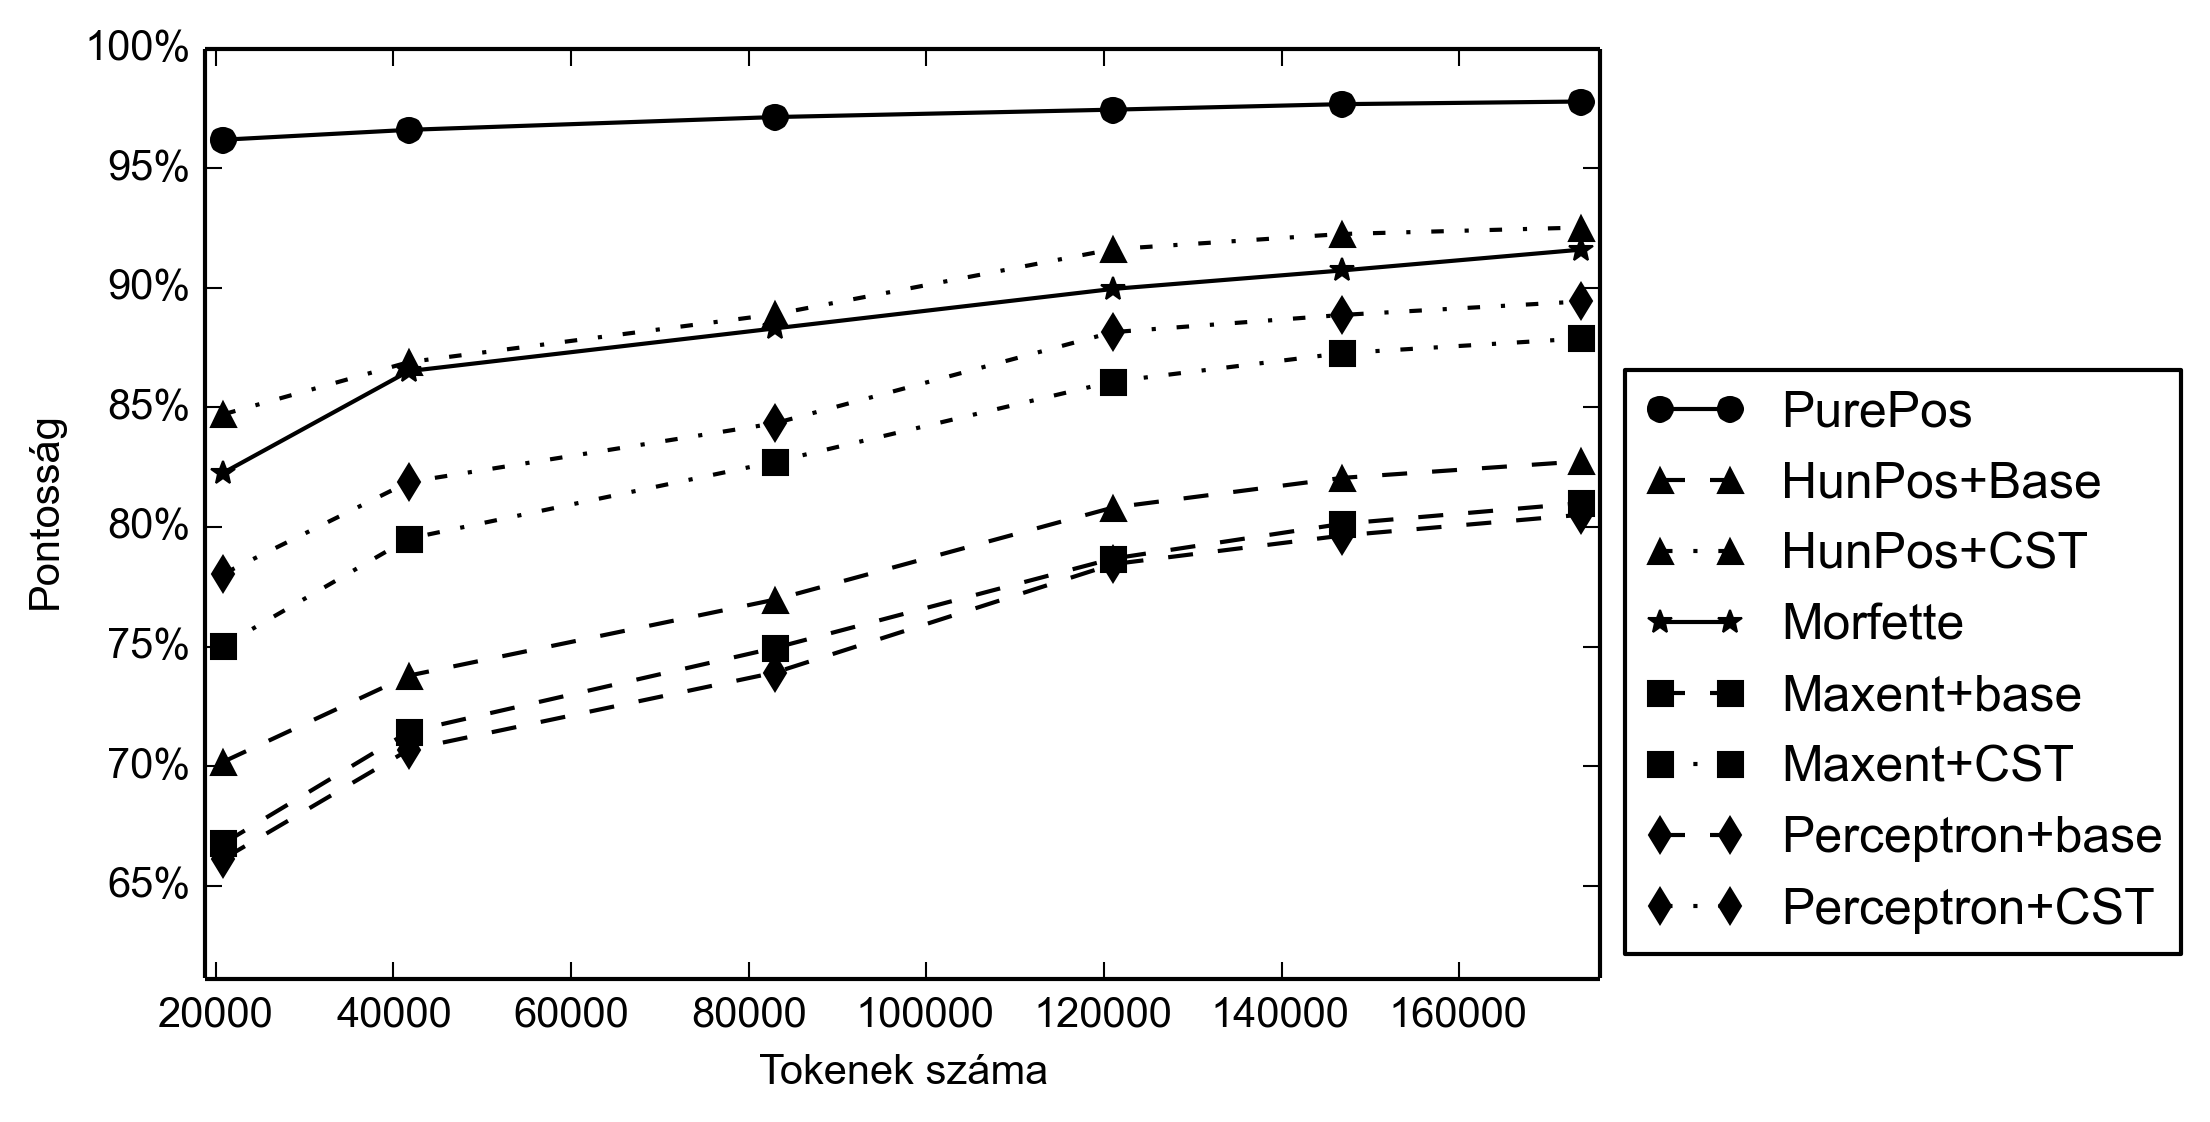
\includegraphics[width=1\textwidth]{MorphTagging/humor_token_hu.png}
  \caption{Morfológiai egyértelműsítő algoritmusok tanulási görbéje}
  \label{fig:humor-token_hu}
\end{figure}

Méréseimmel megmutattam, hogy a bemutatott egyértelműsítő algoritmus kimagasló pontossággal bír magyar nyelv esetén. 
Ehhez a PurePos rendszert a Szeged Korpuszon tanítottam és teszteltem. 
A rendszer ezen szövegek esetén 96,27\%-os szószintű pontosságot nyújt, mely meghaladja más szabadon elérhető eszközök teljesítményét.
Vizsgáltam még az eszköz alkalmazhatóságát olyan esetekben, amikor csak kevés tanítóanyag áll rendelkezésre.
Kimutattam, hogy a PurePos ilyenkor is nagy pontossággal alkalmazható (vö. \ref{fig:humor-token_hu}. ábra). 
Ismertettem még az eljárás egy olyan alkalmazását, ahol a hibrid komponenseinek köszönhetően jelentős mértékben sikerült javítani az eredeti elemzőlánc pontosságán, így gyorsítva a manuális annotációs folyamatot.


\thesisline%%%%%%%%%%%%%%%%%%%%%%%%%%%%%%%%%%%%%%%%%%%%%%%%%%%%%%%%%%%%%%%%%%%%%


Bár a \ref{thes:morf-tagging} tézisben bemutatott algoritmusok magas pontossággal rendelkeznek, megmutattam, hogy ezek teljesítménye tovább növelhető más rendszerekkel való kombinációval. 

\begin{core}
\begin{thesis}
Létrehoztam egy olyan módszert, mely morfológiai egyértelműsítő rendszerek kombinációjával hatékony növeli a címkézés pontosságát magyar nyelv esetén.
A kidolgozott eljárás újdonsága, hogy külön modulban végzi a lemmák és morfoszintaktikai címkék azonosítását, majd azok kimenetét egyesítve határozza meg a morfológiai annotációt.
A módszer példány alapú tanulásra épül és az egyes alrendszereket keresztvalidáción keresztül tanítja.
Méréseimmel alátámasztottam, hogy az ismertetett módszer jelentős mértékben képes növelni a címkézési feladat pontosságát. 
\end{thesis}

\begin{pub}
\cite{Laki2013a,Orosz2013c,Orosz2013d} 
\end{pub}
\end{core}

Első lépésként, kidolgoztam egy új metrikát (OER), amellyel egyértelműsítő rendszerek hibáinak különbözőségét vizsgáltam. 
Ezt felhasználva megmutattam, hogy a HuLaPos rendszer tipikus hibái számottevően eltérnek a PurePos-étól. 

Az általános kombinációs algoritmusok eredményességének részletes vizsgálata után, olyan jellemzőhalmazokat hoztam létre, melyek morfológiailag komplex nyelvek esetében magas pontossággal használhatóak.
Ezt követően kidolgoztam egy olyan eljárást (\ref{fig:comb3_en}. ábra) melyben két külön komponens választja ki a szófaji címkéket, illetve a lemmákat. 
A kombinációs rendszer moduljai keresztvalidáció segítségével tanítják az első szintű osztályozókat, amik példány alapú tanulásra épülnek.

\begin{figure}[H]
  \centering %TODO: magyarul
  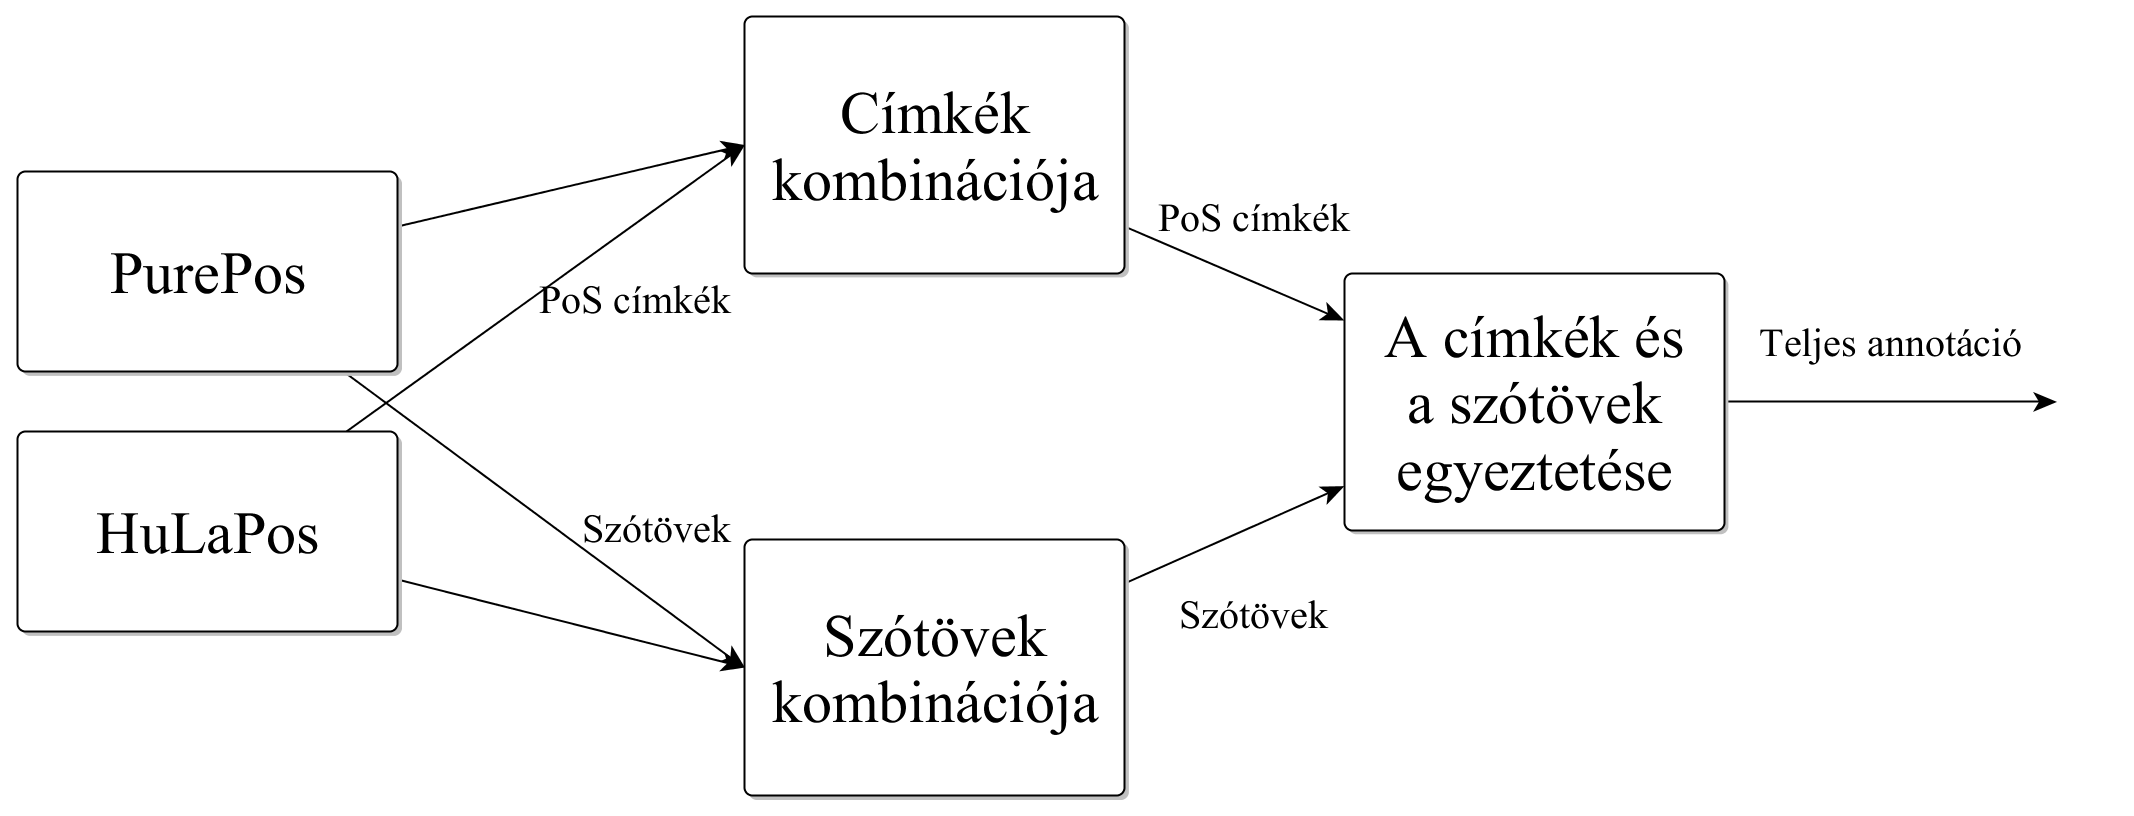
\includegraphics[scale=0.15]{MorphTagging/comb3_hu.png} 
  \caption{A kombinációs rendszer működése}
  \label{fig:comb3_en}
\end{figure}

Méréseimmel megmutattam, hogy az új algoritmus a PurePos hibáinak mintegy 28,90\%-át javítja. 
%Így eredményeimmel igazoltam, hogy egy teljes egyértelműsítő algoritmus pontossága jelentős mértékben javítható egy másik rendszerrel való kombinációval. 

\subsection{Morfoszintaktikai komplexitás automatikus becslése morfológiai egyértelműsítő algoritmusok alkalmazásával}
\label{thes:mlu}

A morfológiai komplexitás mérése fontos eszköze a nyelvfejlődést mérő nyelvészeti kutatásoknak.
Ezt agglutináló nyelvek esetén a megnyilatkozások átlagos morfémában mért hosszával (MLUm) számolják.
Míg angolra és más morfológiailag nem összetett nyelvre léteznek automatikus algoritmusok a feladat megoldására, addig magyarra (és egyéb agglutináló nyelvekre) ezek közvetlenül nem alkalmazhatóak. 
Ezekben az esetekben a megnyilatkozások hosszának mérése csak időigényes manuális számolással végezhető el.

Dolgozatomban megmutattam\footnote{A morfológiai komplexitás becslésének feladatát Mátyus Kingával együtt végeztem. A korpusz manuális címkézése, az annotálás útmutató kidolgozása közös munka eredménye. Az MLUm becslés nyelvészeti alapvetései a társzerző érdeme, míg a folyamat algoritmizálása önálló eredmény.}, hogy a PurePos rendszer egy megfelelő morfológiai elemzővel kiegészülve adekvát alapja egy automatikus morfémaszám-becslő eljárásnak. %, és így kiváltja a fáradtságos emberi munkát. 

\begin{core}
\begin{thesis}
\label{thes:spoken-morf-tagging}
Létrehoztam egy  hibrid morfológiai egyértelműsítő láncot magyar gyermeknyelvi beszédátiratok nagy pontosságú elemzésére. 
Az algoritmus alapját az \ref{thes:morf-tagging} tézisben ismertetett rendszer képezi, amelyet a beszélt nyelv címkézéséhez szükséges szabályokkal adaptáltam. 
Méréseimmel igazoltam, hogy a létrejött elemzési lánc teljesítménye megközelíti az általános nyelvi címkézők eredményességét.
\end{thesis}

\begin{pub}
\cite{Matyus2014,Orosz2014c}
\end{pub}
\end{core}

Mivel a bemutatott morfológiai egyértelműsítő rendszer a Humor elemzőre épül, azt a beszélt nyelvben tipikus jelenségekkel egészítettem ki. 
Ezt követően a PurePos rendszert további szabály alapú eljárásokkal adaptáltam a doménhez.

A lánc pontosságának méréséhez létrehoztunk egy 1000 megnyilatkozásból álló etalon korpuszt, mely a MONYEK \cite{Matyus2014} adatbázis részét képezik. 
Az annotáció folyamatához kidolgoztuk egy az eddigiektől eltérő, beszélt nyelvre adaptált címkekészletet, majd létrehoztunk egy annotálási útmutatót is.

A bemutatott szabály-alapú és sztochasztikus technikák alkalmazásával 96\%-os szószintű pontosságot értem el, mely megközelíti az általános nyelvi egyértelműsítőkét.
Vizsgálataimmal alátámasztottam, hogy a PurePos rendszer nagy pontossággal használható magyar nyelvű beszédátiratok elemzésére. 

%TODO: *specifikus/alapú

\thesisline%%%%%%%%%%%%%%%%%%%%%%%%%%%%%%%%%%%%%%%%%%%%%%%%%%%%%%%%%%%%%%%%%%%%%


\begin{core}
\begin{thesis}
\label{thes:mlu-estimation}
Kifejlesztettem egy olyan új eljárást, amely magyar nyelvű beszédátiratok morfoszintaktikai összetettségét képes automatikusan becsülni.
Az algoritmus a \ref{thes:spoken-morf-tagging} tézisben bemutatott elemzőláncra épülve számolja a megnyilatkozások morfémában mért hosszát. 
Méréseimmel kimutattam, hogy a módszer megfelelően képes helyettesíteni az időigényes manuális számolást.
\end{thesis}

\begin{pub}
\cite{Matyus2014,Orosz2014c}
\end{pub}
\end{core}

Az algoritmus a szavak morfoszintaktikai annotációjára épülve összegzi a megnyilatkozások morfémáit.
A Humor elemző által ismert szavakat annak használatával morfémákra bontja, míg az ismeretlen szóalakokhoz a morfoszintaktikai címke alapján készít becslést.
%Teszi mindezt úgy, hogy közben az MLUm becsléshez nyelvészetileg releváns szabályokat valósít meg.

Az módszer tökéletesítéséhez létrehoztunk egy morfémaszámokat is tartalmazó etalon korpuszt. 
Megmutattam, hogy az automatikus módszer ezen az adathalmazon 0,9901 korrelációs értékkel bír, míg az algoritmus átlagos relatív eltérése  is csupán 4,49\%. 
%Ezzel bebizonyítottam, hogy az összetett eljárás kiválthatja a fáradtságos manuális számolást.
Méréseimmel bebizonyítottam, hogy az eljárás alkalmas az időigényes manuális morfémaszámolás kiváltására.

\subsection{Hatékony előfeldolgozó algoritmusok egy kevés erőforrással rendelkező zajos doménhez}
\label{thes:clin}

Napjainkban egyre több elektronikusan rögzített dokumentum keletkezik klinikai környezetben, melyek nagy mennyiségű eddig el nem érhető közvetett tudást reprezentálnak. 
Mivel létrehozásuk során nem fordítottak kellő figyelmet a szövegek struktúrájának kialakítására és a helyesírási normák betartására, így azok feldolgozása gyakran nem lehetséges létező eszközök közvetlen alkalmazásával. 
Bár angol nyelvre számtalan megoldás született az évek során, a magyar (és más morfológiailag összetett) nyelvű orvosbiológiai szövegek elemzése egy alig vizsgált terület.

% \begin{core}
% \begin{thesis}
% 
% \end{thesis}
% 
% \begin{pub}
% \cite{Orosz2013d, Orosz2014a}
% \end{pub}
% \end{core}


%%%%%%%%%%%%%%%%%%%%%%%
% \thesisline%%%%%%%%%%%%
%%%%%%%%%%%%%%%%%%%%%%%

\begin{core}
\begin{thesis}%{II.1/b}
\label{thes:clin-segment}
Létrehoztam egy olyan hibrid eljárást, mely magyar nyelvű klinikai rekordokat képes magas pontossággal mondatokra és szavakra bontani. 
A módszer alapját egy szabály-alapú szegmentáló algoritmus képezi, amelyet felügyelet nélküli gépi tanulással egészítettem ki. %, melyek hatékonyan képesek javítani a teljesítményén.
Méréseimmel alátámasztottam, hogy a hibrid rendszer által azonosított mondat- és szóhatárok kellően pontosak a gyakorlati alkalmazhatósághoz.
Ezen túl kimutattam még, hogy a magyar nyelvre elérhető algoritmusok közül sem a szabályalapú, sem a gépi tanulást használó rendszerek nem alkalmasak orvosbiológiai szövegek tokenizálására és mondatokra bontására.
\end{thesis}

\begin{pub}
\cite{Orosz2013d, Orosz2014a}
\end{pub}
\end{core}


\begin{figure}[H] %TODO: magyarítás
  \centering
  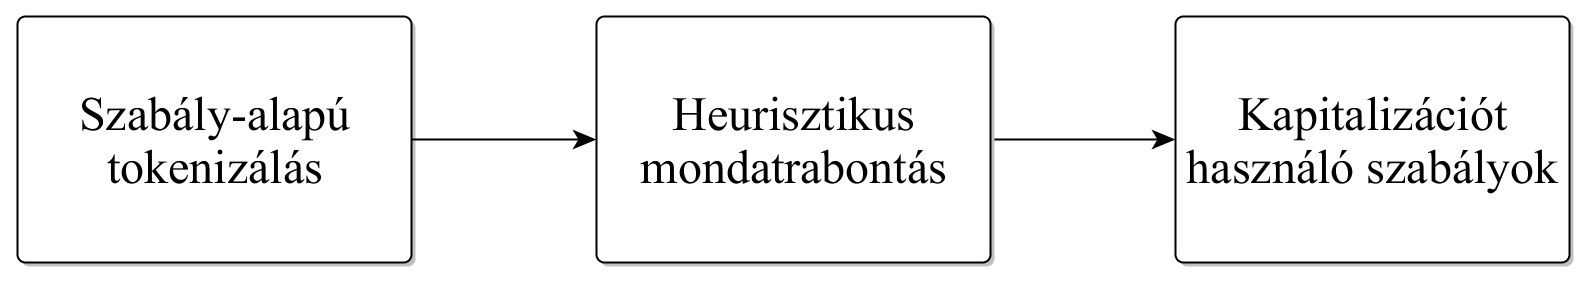
\includegraphics[scale=0.16]{Clinical/clin_segm_arch_hu.png} 
  \caption{A szegmentáló algoritmus részei}
  \label{fig:clin-segment-arch_en}
\end{figure}


A bemutatott szegmentáló algoritmus alapját szabály-alapú, mintaillesztést használó algoritmusok képezik. 
Ezek bár magas pontossággal bírnak, fedésük alacsony, így ezt további heurisztikus eljárásokkal bővítettem.
Megmutattam, hogy a módosított $\log \lambda$ szűrő nagy mértékben képes növelni a rendszer fedését. 
A teljesítmény javításához a szóalakok felszíni jegyein túl, a Humor morfológiai elemzéseit is felhasználtam.

A mérésekhez létrehoztam egy manuálisan javított korpuszt, amin az egyes rendszerek szó- és mondat-szintű pontosságát, fedését és a kombinált $F$-értéket is vizsgáltam.  
Kutatásomban a speciálisan magyar nyelvre fejlesztett rendszereket, illetve egy maximum entrópia módszeren alapuló általánosan használt eszközt is kiértékeltem.

Mérésekkel megmutattam, hogy a mondatrabontás feladatában a legtöbb elérhető rendszer 50\%-os $F$-érték alatt teljesít. 
%Ezek alól csak két eszköz képezett kivételt, de egy részletes elemzésben rávilágítottam, hogy azok kimenete sem alkalmas további feldolgozó rendszerek bemenetéül.
Ezzel szemben méréseimmel azt is alátámasztottam, hogy az új hibrid algoritmus mind a mondatokra mind pedig a szavakra bontás tekintetében 90\% feletti $F$ értéket produkál, így az alkalmas 
%Következésképpen bebizonyítottam, hogy az ismertetett algoritmusok alkalmasak 
magyar nyelvű klinikai dokumentumok szegmentálására.

%%%%%%%%%%%%%%%%%%%%%%%
\thesisline%%%%%%%%%%%%
%%%%%%%%%%%%%%%%%%%%%%%

\begin{core}
\begin{thesis}%{II.2}
\label{thes:clin-pos}
Megmutattam, hogy az \ref{thes:morf-tagging} tézisben ismertetett rendszer, megfelelő adaptációs technikákkal kombinálva alkalmas orvosbiológiai szövegek elfogadható minőségű morfológiai egyértelműsítésére. 
Méréseimmel kimutattam, hogy az ismertetett szabály-alapú és statisztikai doménadaptációs módszerek jelentős mértékben javítanak az elemzési lánc pontosságán.
\end{thesis}

\begin{pub}
\cite{Orosz2013,Orosz2014b} 
\end{pub}
\end{core}

Az eljárás a Humor morfológiai elemző egy bővített változatára és a PurePos egyértelműsítő rendszerre épül. 
Dolgozatomban feltártam az így kapott alaprendszer tipikus hibáit és az algoritmus számos hiányosságát orvosoltam doménspecifikus szabályok alkalmazásával. 

A mérések elvégzéséhez létrehoztam egy etalon korpuszt, melynek morfológiai annotációját manuálisan javítottam. 
Megmutattam, hogy a közreadott rendszer szószintű pontossága (93,73\%) jelentősen meghaladja az alapjául szolgáló eredeti rendszer teljesítményét (88,09\%). 

Ismertettem még, hogy a bemutatott klinikai dokumentumokat szegmentáló és egyértelműsítő eljárások hibái a rövidítések kezelésének nehézségeiből fakadtak.
Így a jövőben indokolt lehet egy olyan módszer kidolgozása, mely a két feladatot egyszerre célozza meg.

\let\thesubsection=\oldthesubsection
